\subsubsection{الگوی \lr{Channel}}
\label{archChannelSec}
\begin{RTL}
الگوی معماری کانال \cite{ref4} در دو موقعیت اصلی مفید است:
زمانی که داده‌ها در یک جریان داده به صورت ترتیبی از طریق
چندین مرحله تبدیل می‌شوند و زمانی که اطمینان از قابلیت اطمینان
بالا و ایمنی در برنامه‌های حیاتی مورد نیاز است.
این الگو یک کانال را به عنوان یک لوله در نظر می‌گیرد که
داده‌ها را به صورت ترتیبی پردازش می‌کند و هر عنصر داخلی
یک عملیات ساده انجام می‌دهد. چندین کانال می‌توانند با پردازش همزمان
عناصر مختلف داده‌ها توان عملیاتی را افزایش دهند و از طریق تکرار
قابلیت اطمینان و ایمنی را بهبود بخشند. این الگو به ویژه برای الگوریتم‌هایی
که نیاز به تبدیل‌های مکرر دارند موثر است و امکان پردازش
موازی کارآمد و تحمل خطا را فراهم می‌کند.
\end{RTL}
\begin{figure}[h!]
\centering
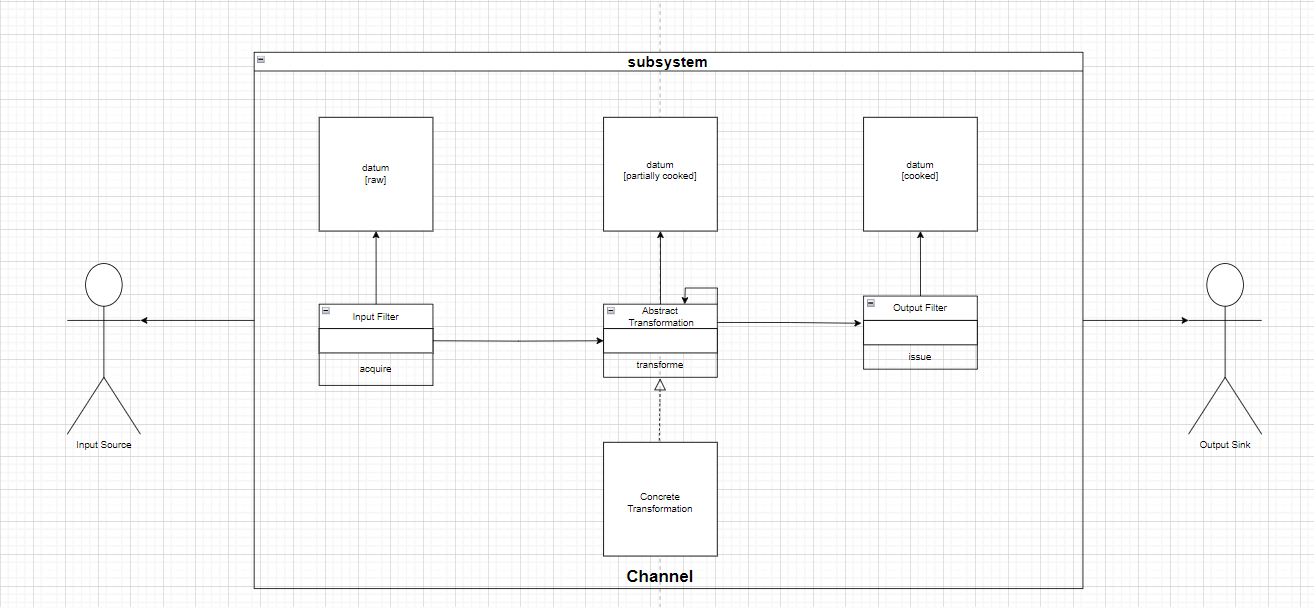
\includegraphics[scale=0.5]{images/first/channel.png}
\caption{ساختار الگوی \lr{Channel}}
\end{figure}